\documentclass[12pt]{article}
\usepackage{graphicx}
\usepackage{amssymb}
\usepackage{epstopdf}
\usepackage{amsmath}
\usepackage{multicol}
\usepackage{tcolorbox}
\usepackage{geometry}
\usepackage{enumitem}
\usepackage{fancyhdr}

\DeclareGraphicsRule{.tif}{png}{.png}{`convert #1 `dirname #1`/`basename #1 .tif`.png}

\textwidth = 6.5 in
\textheight = 9 in
\oddsidemargin = 0.0 in
\evensidemargin = 0.0 in
\topmargin = -23pt
\headheight = 0.0 in
\headsep = 0.0 in
\parskip = 0.2in
\parindent = 0.0in
\pagestyle{fancy}
\pagenumbering{gobble}

\newtheorem{theorem}{Theorem}
\newtheorem{corollary}[theorem]{Corollary}
\newtheorem{definition}{Definition}
%\includegraphics [height=50mm, width=50mm]{PathInt.jpg}
\title{Title} 

\begin{document}


 Name:
 \begin{center}\large{6.1 Antiderivatives Graphically}\end{center}

\begin{enumerate}

\item This is a graph of $F'(x)$. \\
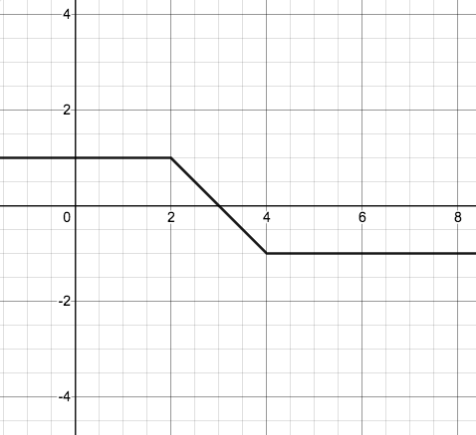
\includegraphics[scale=0.5]{6_1_1}

	\begin{enumerate}
	\item Starting at $F(0)=0$, sketch a graph of $F(x)$. Be as accurate as you can. 
	\item Let's do it again with a different starting point. Starting at $F(0)=-2$, sketch a graph of $F(x)$.
	\item Check your work using Desmos.
	\item Summarize your findings: If you are given a graph of $F'(x)$, how can you construct the original function $F(x)$?
	\vfill
	\item Are antiderivatives unique? What is similar about all of the antiderivatives of $F(x)$?
	\vfill
	\end{enumerate}
	
\newpage

$\hspace{10px}$\\
	
\item This is a graph of $G'(x)$. \\
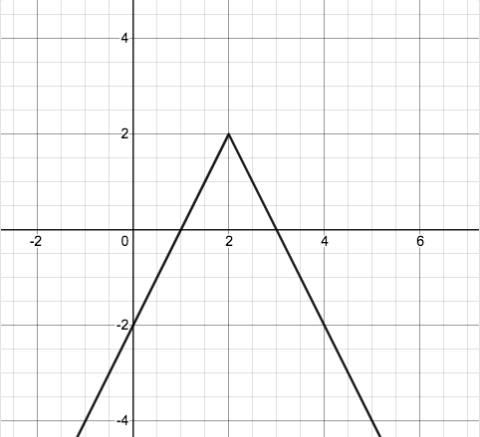
\includegraphics[scale=0.35]{6_1_2}

	\begin{enumerate}
	\item Sketch $G(x)$ where $G(0)=0$.
	\item Where is $G(x)$ increasing? Why?
	\vfill
	\item Where is $G(x)$ concave up? Why?
	\vfill
	\end{enumerate}



\item The graph of $h(x)=H'(x)$ is shown. \\
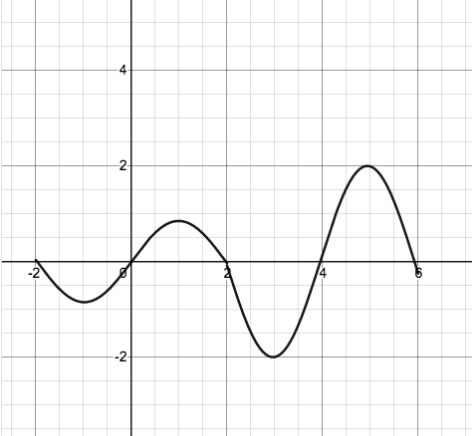
\includegraphics[scale=0.35]{6_1_3}
	\begin{enumerate}

	\item Where is $H(x)$ increasing? Why?
	\vfill
	\item Where is $H(x)$ concave up? Why?
	\vfill
	\item Sketch $H(x)$ where $H(0)=0$.
	\end{enumerate}


\end{enumerate}
\end{document}
%%%%%%%%%%%%%%




